\documentclass[UTF8]{ctexart}
\usepackage{bookmark}
\usepackage{geometry}
\usepackage{hyperref}
\geometry{a4paper,scale=0.8}
\usepackage{ctex}
\usepackage{booktabs}
\usepackage{array}
\usepackage{fancyhdr}
\usepackage{physics}
\pagestyle{fancy}
\fancyhf{}
\renewcommand\footrulewidth{1pt}
\lhead{\textit{王铠泽}}
\rhead{\textit{PB18020766}}
\chead{\href{mailto:volar@mail.ustc.edu.cn}{\textit{volar@mail.ustc.edu.cn}}}
\rfoot{\href{http://en.ustc.edu.cn/}{\textit{中国科学技术大学}}}
\lfoot{\textit{\today}}
\usepackage{graphicx}
\usepackage{float}
\usepackage{subfigure}
\fancyfoot[C]{\textit{\thepage}}


\begin{document}

	\centering\textbf{\LARGE{计算物理A第十九次作业}}
	
	
	\textit{王铠泽}\qquad\textit{ PB18020766}
	
		
	\section{作业题目}
	
	\begin{itemize}
		\item 用 Numerov 法求解一维定态薛定谔方程在一个对称势阱
		(势能函数 V(x)可任意设置)中的基态和激发态的能量本征值。画出
		能量本征值及其附近的波函数。
		
		$$\left( -\frac{\hbar^2}{2m}\frac{\partial^2}{\partial x^2}+V(x)\right) \psi(x)=E\psi(x)$$
	\end{itemize}
	
	\section{实现方法和原理}
	
	\begin{itemize}
		\item Numerov方法
		
		对于如下形式的微分方程:
		
		$$\phi''(x)=F(\phi,x)=f(x)\phi(x)$$
		
		做变量代换:
		
		$$y(x)=\left[ 1-\frac{h^2f(x)}{12}\right]\phi(x) $$
		
		得到如下迭代格式:
		
		$$\Rightarrow y_{n+1}=2y_{n}-y_{n-1}+h^2f_n\phi_n+O(h^6)$$
		
		$$\Rightarrow \phi_{n+1}=\frac{2y_{n}-y_{n-1}+h^2f_n\phi_n}{1-\frac{h^2f_n}{12}}$$
		
		\item 打靶法
		
		在求解边值问题时,常用的方法是先给出预估的能量$E$值,然后根据参数计算的结果进行调整。
		
			\begin{figure}[H]
				\centering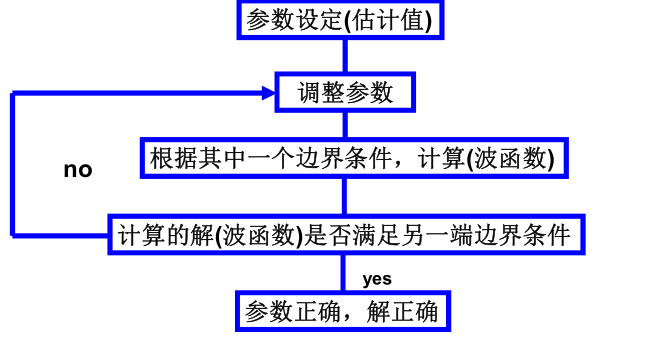
\includegraphics[width=4in]{1}
				\caption{打靶法算法描述}
				\end{figure}
			
		在本次实验中,由于理论上边界是无穷大处为零,所以取足够大的$x_0$作为截断,边界条件变为$\psi(\pm x_0)=0$。本次实验中采取的对称势为谐振子势能加上四阶项微扰:
		
		$$V(x)=\frac{1}{4}x^2+\epsilon x^4(\epsilon<<1)$$ 
		
		薛定谔方程简化为:
		
		$$\left( -\frac{\partial^2}{\partial x^2}+\frac{1}{4}x^2+\epsilon x^4\right) \psi(x)=E\psi(x)$$
		
		对于基态和第一激发态的能量预估值$E_{G0},E_{G1}$分别以理想无微扰的谐振子势能计算得到:
		
		$$E_{G0}=0.5,E_{G1}=1.5$$
		
		其零阶近似解为:
		
		$$\psi_0^{(0)}(x)=\left( \frac{1}{2\pi}\right) ^{1/4}exp(-\frac{x^2}{4})$$
		
		$$\psi_1^{(0)}(x)=\left( \frac{1}{2\pi}\right) ^{1/4}x \,exp(-\frac{x^2}{4})$$
		
		可以取特征截断长度为$x_0=6$。本次实验采取$\epsilon=\frac{1}{1000},\frac{2}{1000},\frac{3}{1000}$,$h=1.2\times10^{-3}$,参数每一次初始变化步长$\Delta E=0.01$,此后作为可调节变量不断缩小,当上一个循环的$\psi(x_0)$和本循环的$\psi(x_0)$异号时,$\Delta E=\Delta E/10$。
		
		$$f(x)=\frac{1}{4}x^2+\epsilon x^4-E_G$$
		
		\item 理论结果
		
		理论上能量的一阶微扰为:
		
		$$\delta E=\bra{\psi^{(0)}}\epsilon x^4\ket{\psi^{(0)}}$$
		
		$$E_0^{(1)}=E_0^{(0)}+\delta E_0=0.5+3\epsilon$$
		$$E_1^{(1)}=E_1^{(0)}+\delta E_0=1.5+15\epsilon$$
		
		当$\epsilon=\frac{1}{100}$时还是比较接近微扰的,具体见下面两个势能项的对比:
		
			\begin{figure}[H]
					\centering  %图片全局居中
					\subfigure[$\epsilon=0.01$]{
						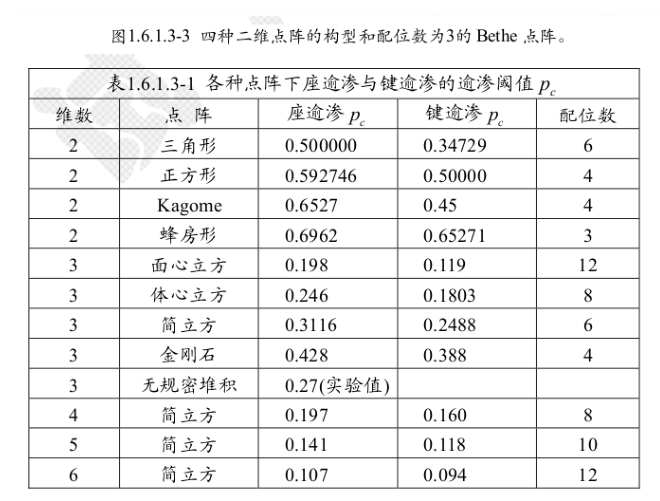
\includegraphics[width=0.45\textwidth]{../result/3}}
					\subfigure[所有$\epsilon$对比]{
						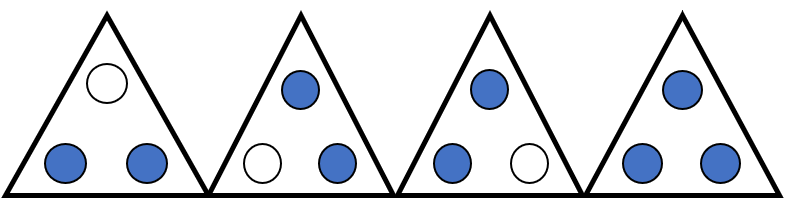
\includegraphics[width=0.45\textwidth]{../result/2}}
					\caption{势能曲线对比}
			\end{figure}
			
	当$\epsilon=0.01$,四次方项在$x=4$处和二次方项以及能相比大小了,此时大约是$2\sigma$,还尚能算做微扰,其余的两个微扰处理出来的理论值应该误差会比较大,这可以参见后续的计算结果讨论。
	
		
	\end{itemize}
	
	\section{程式说明}
	
	\begin{itemize}
		\item Numerov.c
		
		这是一个能用于计算对称势能下的定态薛定谔方程能量本征值和波函数的程式,结果以文件形式输出。运行结束时会有边界上$\psi(x_0)$大小和能量本征值的提示。
		
		\item ground\_state\_1/2/3.txt
		
		这三个文件分别对应着$\epsilon=0.01,0.02,0.03$的基态能量和波函数输出。左一列是位置$x$,右一列是波函数的值$\psi(x)$。
		
		\item 1st\_excited\_state\_1/2/3.txt
		
		这三个文件分别对应着$\epsilon=0.01,0.02,0.03$的第一激发态能量和波函数输出。左一列是位置$x$,右一列是波函数的值$\psi(x)$。
		
		\item 2nd\_excited\_state.txt
		
		这三个文件分别对应着$\epsilon=0.03$的第二激发态能量和波函数输出。左一列是位置$x$,右一列是波函数的值$\psi(x)$。
		
		
		
	\end{itemize}
	
	\section{计算结果}
	
	\subsection{能量计算}
		
	\begin{flushleft}
		采用$Numerov$方法和打靶法得到的能量本征值如下:
	\end{flushleft}
	
		
		\begin{table}[H]
				\centering
				\begin{tabular}{@{}cccc@{}}
					\toprule
					$\varepsilon$& $E_{0}$ &$E_{1}$  &$E_{2}$ \\ \midrule
					0.00&  0.500000&  1.500000&  2.500000  \\
					0.01&  0.526734&  1.626748&  --  \\
					0.02&  0.549072&  1.725986&  --  \\
					0.03&  0.568652&  1.810017&  3.228912  \\ \bottomrule
				\end{tabular}
			\caption{计算结果}
	\end{table}

	\begin{flushleft}
		其中$\epsilon=0.00$是未加微扰的理想结果,不是计算得到的。
	\end{flushleft}
		
		

	\begin{flushleft}
		
		在一阶微扰近似下:
		
			\begin{table}[H]
			\centering
			\begin{tabular}{@{}cccccccccc@{}}
				\toprule
				$\varepsilon$& $E_{0}$ &$E_{1}$  &$E_{2}$ & $E_{0}^{(1)}$ &$E_{1}^{(1)}$  &$E_{2}^{(1)}$&$err_0(\%)$&$err_1(\%)$&$err_2(\%)$  \\ \midrule
				0.01&  0.526734&  1.626748&  -- &0.53&1.65&--&0.62&1.41&-- \\
				0.02&  0.549072&  1.725986&  --  &0.56&1.80&--&2.13&4.11&--\\
				0.03&  0.568652&  1.810017&  3.228912&0.59&1.95&3.67&3.62&7.12&12.02  \\ \bottomrule
			\end{tabular}
			\caption{和理想的非简并一阶微扰的比较}
		\end{table}
	
	可以看出,$\varepsilon=0.01$和微扰计算较为一致,而且随着能级升高,越来越偏离微扰计算。另一方面一阶微扰所计算得到的能量都偏高,这和我们在量子力学课上学习得到的结果是相互一致的。
	
	还有值得一提的是$\varepsilon$增大时会越来越偏离微扰计算的范畴,当$\varepsilon=0.03$时已经出现很大的偏差,此时当作微扰计算很可能会有问题。笔者尝试计算这种情况下的二阶微扰能量,发现并不收敛。
	
	\end{flushleft}

	
	\subsection{波函数计算}
	
	\begin{flushleft}
		采用$Numerov$方法计算得到的波函数如下:
		
			\begin{figure}[H]
				\centering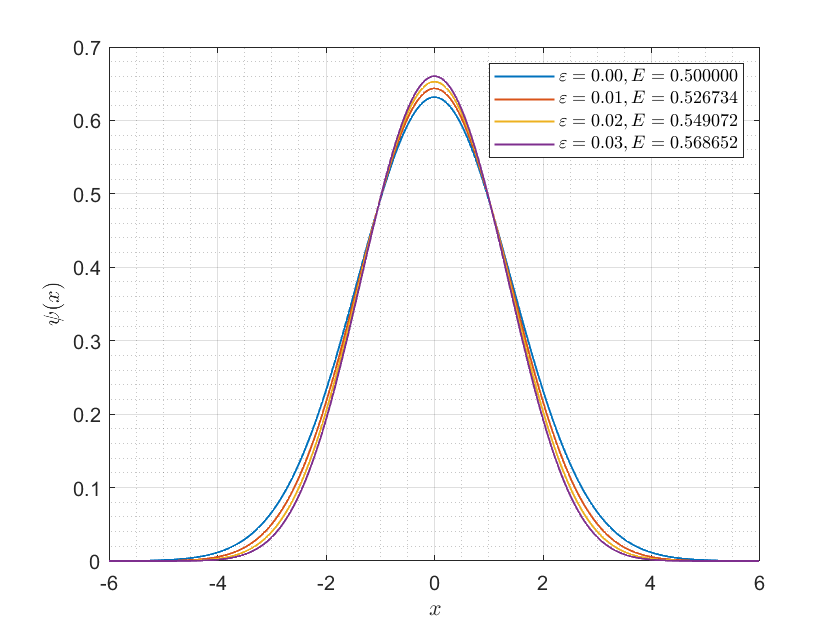
\includegraphics[width=5in]{../result/ground}
				\caption{不同$\varepsilon$下的基态波函数}
			\end{figure}
		
	可以看出随着$\varepsilon$,即微扰的增大,波函数趋于更加局域化,更加集中在$x=0$的附近,展宽更小。这也是符合物理图像的,当加入四阶势能,等于再引入一个三次方正比的吸引力,使得粒子运动更加趋于局域化。
	
	第一,第二激发态的波函数如下:
	
		\begin{figure}[H]
		\centering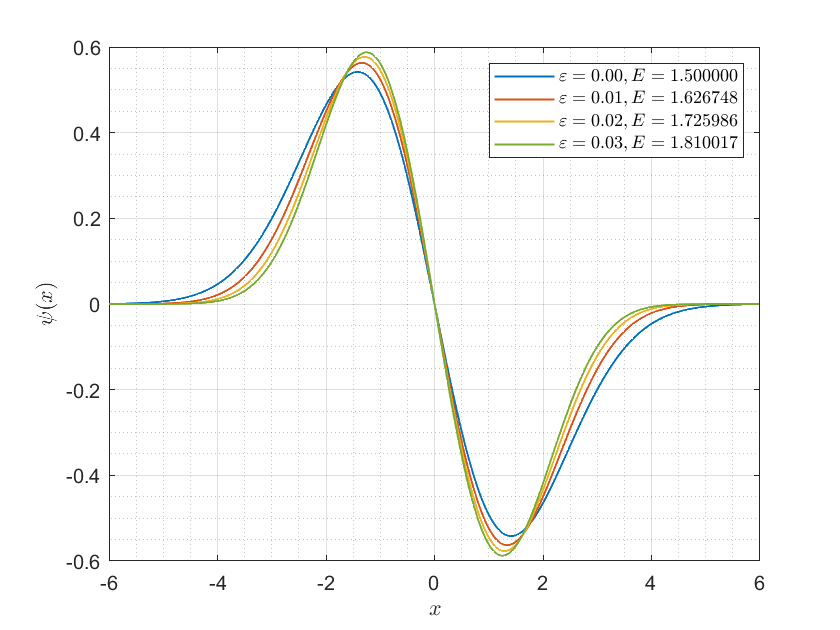
\includegraphics[width=5in]{../result/1st_excited}
		\caption{不同$\varepsilon$下的第一激发态波函数}
	\end{figure}	
	
		\begin{figure}[H]
		\centering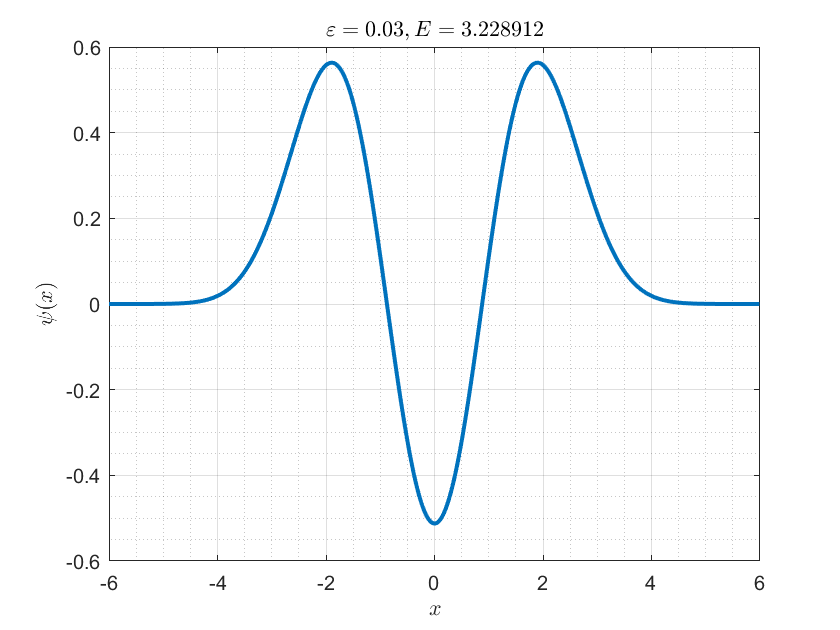
\includegraphics[width=5in]{../result/2nd_excited}
		\caption{$\varepsilon=0.03$下的第二激发态波函数}
	\end{figure}	
		
	激发态的波函数也体现出和基态类似的局域化的特征,符合物理直觉。	
		
	\end{flushleft}
	
	
	
	
%	\begin{table}[H]
%			\centering
%			\begin{tabular}{@{}lllll@{}}
%				\toprule
%				12412& 421342 &41232  & 412231 &  \\ \midrule
%				111&  333&  4324&  312&  \\
%				1323&  132&  132&  123&  \\
%				123&  1323&  1231&  312&  \\ \bottomrule
%			\end{tabular}
%		\end{table}

%	\begin{figure}[H]
%	\centering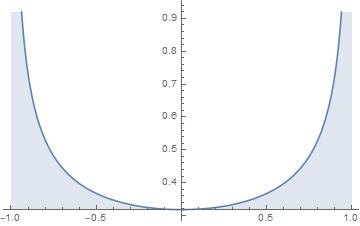
\includegraphics[width=2in]{1.jpg}
%	\caption{something}\label{fig:1}
%	\end{figure}
%		
%	\begin{figure}[H]
%		\centering  %图片全局居中
%		\subfigure[name1]{
%			\label{Fig.sub.1}
%			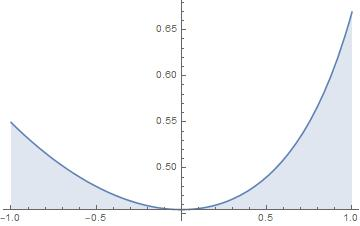
\includegraphics[width=0.45\textwidth]{2.jpg}}
%		\subfigure[name2]{
%			\label{Fig.sub.2}
%			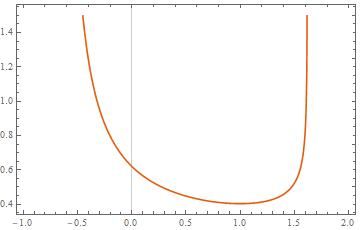
\includegraphics[width=0.45\textwidth]{3.jpg}}
%		\caption{Main name}
%		\label{Fig.main}
%	\end{figure}

	\section{总结}

	\begin{itemize}
		\item $Numerov$法和打靶法是解决边值问题,特别是薛定谔方程的基本方法,能够得到比较理想的结果。
		
		\item 打靶法的能量改变步长应该也要随着程式进行来调节,这样才能得到正确的能量本征值,不然可能会把第一激发态能计算成更高激发态能量,这是由于步长过长导致的。
		
		\item 打靶法的运行效率较低,应该有更加优化的数值方法。
	\end{itemize}

\end{document}